\chapter{Các model nâng cao trong xử lý dữ liệu dạng văn bản}
\label{Chapter4}
\section{Tại sao cần các phương pháp này ?}

Các phương pháp trích xuất đặc trưng truyền thống (dựa trên số lượng) cho dữ liệu văn bản liên quan đến họ phương pháp rất phổ biến là Bag of Words hay bao gồm cả tần số như TF-IDF, N-gram... 

Mặc dù chúng đều là các phương pháp hiệu quả để trích xuất đặc trưng từ văn bản, nhưng do bản chất vốn có của các mô hình đó chỉ là xét trên các từ không có cấu trúc, như vậy chúng ta sẽ mất các thông tin bổ sung như ngữ nghĩa, cấu trúc, trình tự và ngữ cảnh xung quanh các từ gần đó mỗi tài liệu văn bản

Các mô hình nâng cao này có thể trích xuất được các thông tin sâu hơn có thể bao quát được cho cả các từ, thường được gọi là word embeddings.

\section{Mô hình Word2Vec}
Mô hình này được Google rạo ra vào năm 2013 và là mô hình sử dụng deep learning để tính toán và tạo ra các vectơ biểu diễn các từ và bao gồm được cả các tương đồng về ngữ cảnh và ngữ nghĩa của từ đó.

Về cơ bản, đây là mô hình học không giám sát, có thể áp dụng được cho những tập văn bản lớn, tạo ra vốn từ vựng và tạo ra embedding trong không gian vecto cho mỗi từ vựng đó.

Thông thường kích thước của vectơ embeddings và tổng số vectơ là kích thước của không gian từ vựng. Điều này làm cho số chiều của không gian vectơ này thấp hơn rất nhiều so với không gian vectơ được tạo ra bởi mô hình \textbf{Bag of Words} truyền thống.

Có hai kiến trúc khác nhau có thể sử dụng để tạo ra các vectơ embedding này bao gồm \cite{WEBSITE:17} \cite{WEBSITE:18}:
\begin{itemize}
	\item Mô hình \textbf{Continous Bag of Words (CBOW)}
	\item Mô hình \textbf{Skip-gram}
\end{itemize} 


\section{Mô hình Continuous Bag of Words (CBOW)}

Mô hình CBOW sẽ cố gắng dự đoán từ trung tâm (center word hoặc target word) dựa trên ngữ cảnh được tạo ra từ các từ xung quanh nó (surrounding words)

Chúng ta hãy xem xét một câu đơn giản \textbf{"the quick brown fox jumps over the lazy dog"}, chúng ta có thể có các cặp \textbf{ (context-window, target-word)} nếu chọn \textbf{context-window = 2} ta sẽ có \textbf{ ([quick, fox], brown), ([the, brown], quick), ([the, dog], lazy)}. Như vậy ta có thể dự đoán \textbf{target-word} dựa trên \textbf{context-window} như sau \ref{CBOW} \cite{WEBSITE:19}.


\begin{figure}[h!]
	\centering
	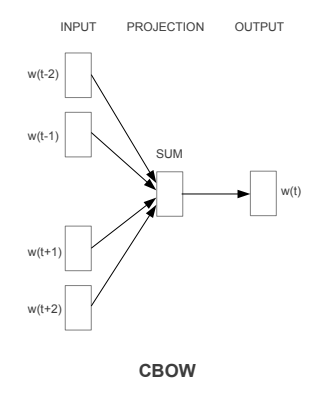
\includegraphics[width=0.8\textwidth]{
		CBOW.png
	}
	\caption[Mô hình CBOW]{
		Mô hình CBOW \label{CBOW}
	}
\end{figure}

\section{Xây dựng mô hình Continuous Bag of Words (CBOW)}

\textbf{ Việc xây dựng mô hình sẽ tập trung vào bốn bước sau}:
\begin{enumerate}
	\item \textbf{Xây dựng tập từ vựng}
	\item \textbf{Xây dựng CBOW generator (bao gồm các cặp [context-window, target-word])}
	\item \textbf{Xây dựng kiến trúc mô hình CBOW}
	\item \textbf{Huấn luyện mô hình}
	\item \textbf{Thu được embedding của các từ}			
\end{enumerate}

\subsection{Xây dựng tập từ vựng}
\lstinputlisting[style=codePython]{"Code/buildVocab.py"}
\textbf{Kết quả}:
\lstinputlisting[style=plaintext]{"Code/vocab.txt"}

\subsection{Xây dựng CBOW generator (bao gồm các cặp [context-window, target-word]}
\lstinputlisting[style=codePython]{"Code/buildCBOWgenerator.py"}
\textbf{Kết quả}:
\lstinputlisting[style=plaintext]{"Code/pairGenerator.txt"}

\subsection{Xây dựng kiến trúc mô hình CBOW}
\lstinputlisting[style=codePython]{"Code/buildCBOWDeep.py"}

\subsection{Huấn luyện mô hình}
\lstinputlisting[style=codePython]{"Code/TrainCBOW.py"}
\textbf{Kết quả}:
\lstinputlisting[style=plaintext]{"Code/CBOWRes.txt"}

\subsection{Thu về Embedding Words}
\lstinputlisting[style=codePython]{"Code/getWordsEmbeddings.py"}
\textbf{Kết quả}: \ref{CBOWRes}
\begin{figure}[h!]
	\centering
	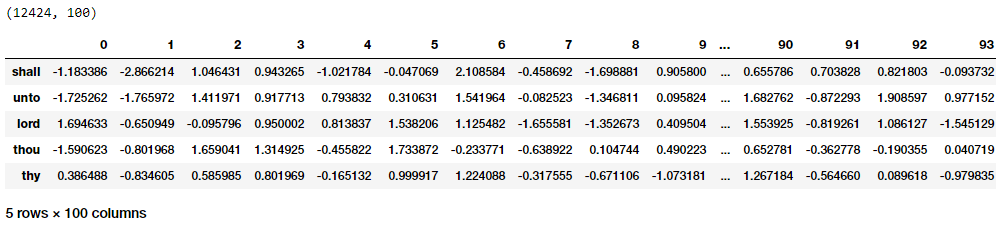
\includegraphics[width=1\textwidth]{
		CBOWRes.png
	}
	\caption[Embedding Words]{
		Embedding Words \label{CBOWRes}
	}
\end{figure}



